\documentclass[convert]{standalone}

\usepackage{tikz}
\usepackage{graphicx}
\pagestyle{empty}

% INT_AY22_L35-Fig01_Circle_polygon_approx.png

\begin{document}
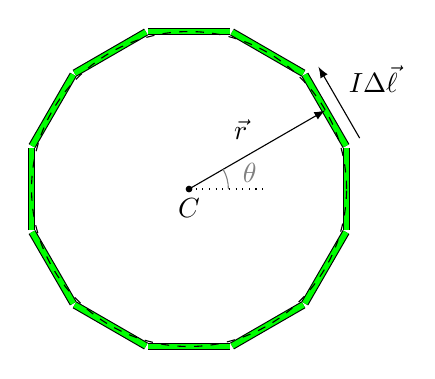
\begin{tikzpicture}[> = latex]

	% Definitions
	
	\def\R{2}		% Circle radius
	\def\N{12} 		% Number of polygonal sides
	
	% Polygon segments
	
	\foreach \Q in {0, 30, ..., 330}
	{
		
		\coordinate (left) at ({\R * cos(\Q) - 3.14 * \R / \N * sin(\Q)}, {\R * sin(\Q) + 3.14 * \R / \N * cos(\Q)});
		\coordinate (right) at ({\R * cos(\Q) + 3.14 * \R / \N * sin(\Q)}, {\R * sin(\Q) - 3.14 * \R / \N * cos(\Q)});
		
		\draw [double = green, double distance = 2 pt] (left) -- (right);
	}
	
	% Vectors for Biot-Savart law
	
	\draw [->] (0, 0) -- node [above left] {${\vec r}$} (30 : \R);
	\draw [->] ({1.1 * \R * cos(30) + 3.14 * \R / \N * sin(30)}, {1.1 * \R * sin(30) - 3.14 * \R / \N * cos(30)}) -- node [above right] {$I \Delta {\vec \ell}$}
			({1.1 * \R * cos(30) - 3.14 * \R / \N * sin(30)}, {1.1 * \R * sin(30) + 3.14 * \R / \N * cos(30)});

	% Actual circle
	
	\draw [dashed] (0, 0) circle (\R);
	
	% Angle indicator
	
	\draw [dotted] (0, 0) -- (0.5 * \R, 0);
	\draw [thin, gray] (0.25 * \R, 0) arc (0 : {360 / \N} : 0.25 * \R);
	\node [gray] at ({180 / \N} : {0.4 * \R}) {$\theta$};
	
	% Center of circle
	
	\filldraw (0, 0) circle (1 pt) node [below] {$C$};

\end{tikzpicture}
\end{document}